\begin{figure}[h!]
  \centering
  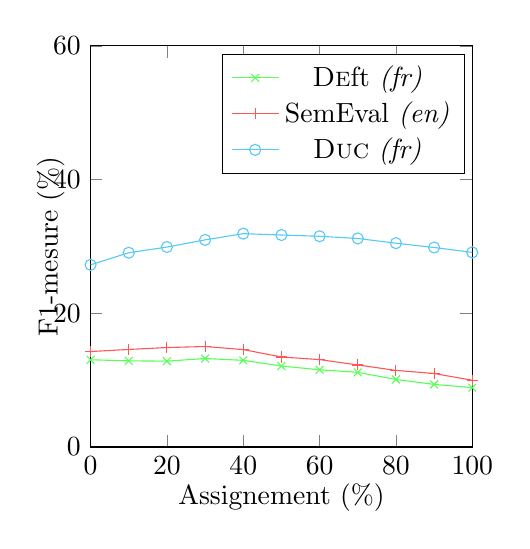
\begin{tikzpicture}
    \pgfkeys{/pgf/number format/.cd, fixed}
    \begin{axis}[x=0.0040\linewidth,
                 xtick={0, 20, ..., 100},
                 xmin=0,
                 xmax=100,
                 xlabel=Assignement (\%),
                 x label style={yshift=.34em},
                 y=0.007\linewidth,
                 ytick={0, 20, ..., 100},
                 ymin=0,
                 ymax=60,
                 ylabel=F1-mesure (\%),
                 y label style={yshift=-1.1em}]
      \addplot[green!66, mark=x] coordinates{
        (0, 13.0470)
        (10, 12.8868)
        (20, 12.8409)
        (30, 13.2342)
        (40, 12.9643)
        (50, 12.1117)
        (60, 11.5492)
        (70, 11.1649)
        (80, 10.1043)
        (90, 9.3643)
        (100, 8.8794)
      };
      \addplot[red!66, mark=+] coordinates{
        (0, 14.2790)
        (10, 14.5905)
        (20, 14.8776)
        (30, 15.0293)
        (40, 14.5713)
        (50, 13.4616)
        (60, 13.0731)
        (70, 12.2721)
        (80, 11.4582)
        (90, 10.9929)
        (100, 9.9841)
      };
      \addplot[cyan!66, mark=o] coordinates{
        (0, 27.2447)
        (10, 29.0553)
        (20, 29.9039)
        (30, 30.9763)
        (40, 31.9071)
        (50, 31.7050)
        (60, 31.5150)
        (70, 31.1887)
        (80, 30.4816)
        (90, 29.8382)
        (100, 29.1068)
      };
      \legend{\textsc{De}ft \textit{(fr)}, SemEval \textit{(en)}, \textsc{Duc} \textit{(fr)}};
    \end{axis}
  \end{tikzpicture}
  \caption{Comportement de TopicCoRank en fonction du taux d'assignement
           \label{fig:assignment_variations}}
\end{figure}

